Wanneer we het convergentie gedrag bekijken van de Ritz waarden valt op dat de meest extreme eigenwaarde (zie \ref{arnoldi_1_100_it}) het snelste convergeert. De andere eigenwaarde liggen dicht bij elkaar geclusterd en convergeren veel langzamer (bv. \ref{arnoldi_2_150_it} haalt na 150 iteraties nog altijd maar een precisie van $10^{-5}$, nog lagere extremen gaan uiteraard nog langzamer (\ref{arnoldi_3_150_it} en \ref{arnoldi_4_150_it}).
\begin{figure}[H]
  \centering
  \subfloat[arnoldi 1, 100 iteraties]{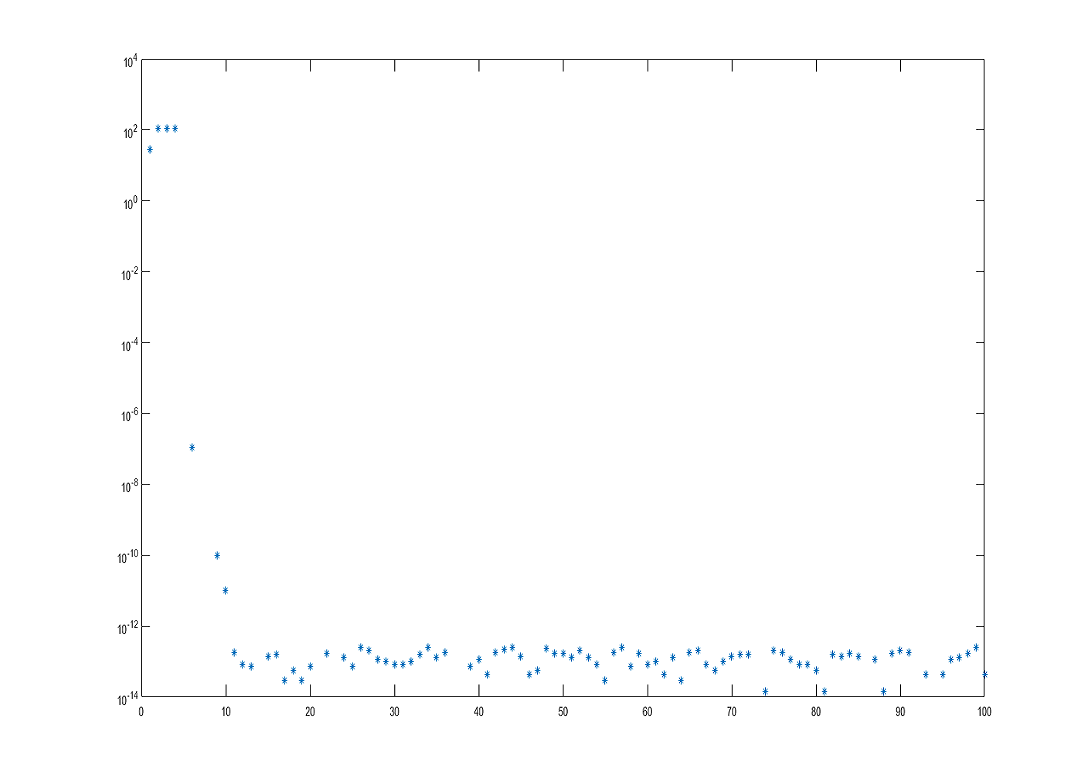
\includegraphics[width=0.5\textwidth]{Tekeningen/arnoldi_1_eig}\label{arnoldi_1_100_it}}
  \hfill
  \subfloat[arnoldi 1, 150 iteraties]{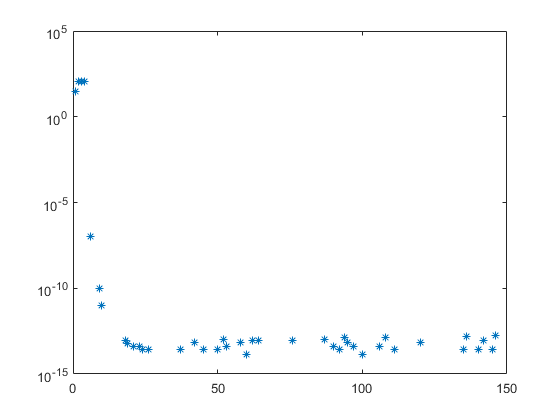
\includegraphics[width=0.5\textwidth]{Tekeningen/arnoldi_1_eig_150it}\label{arnoldi_1_150_it}}
\end{figure}

\begin{figure}[H]
  \centering
  \subfloat[arnoldi 2, 100 iteraties]{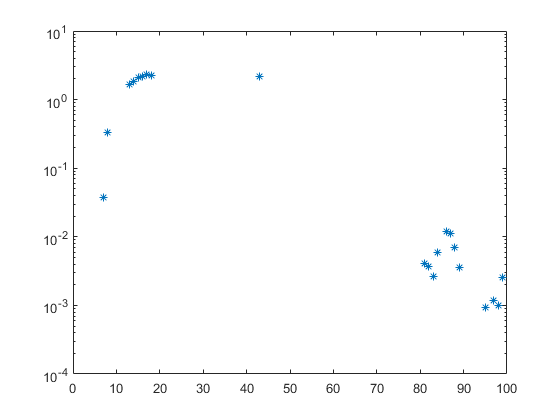
\includegraphics[width=0.5\textwidth]{Tekeningen/arnoldi_2_eig}\label{arnoldi_2_100_it}}
  \hfill
  \subfloat[arnoldi 2, 150 iteraties]{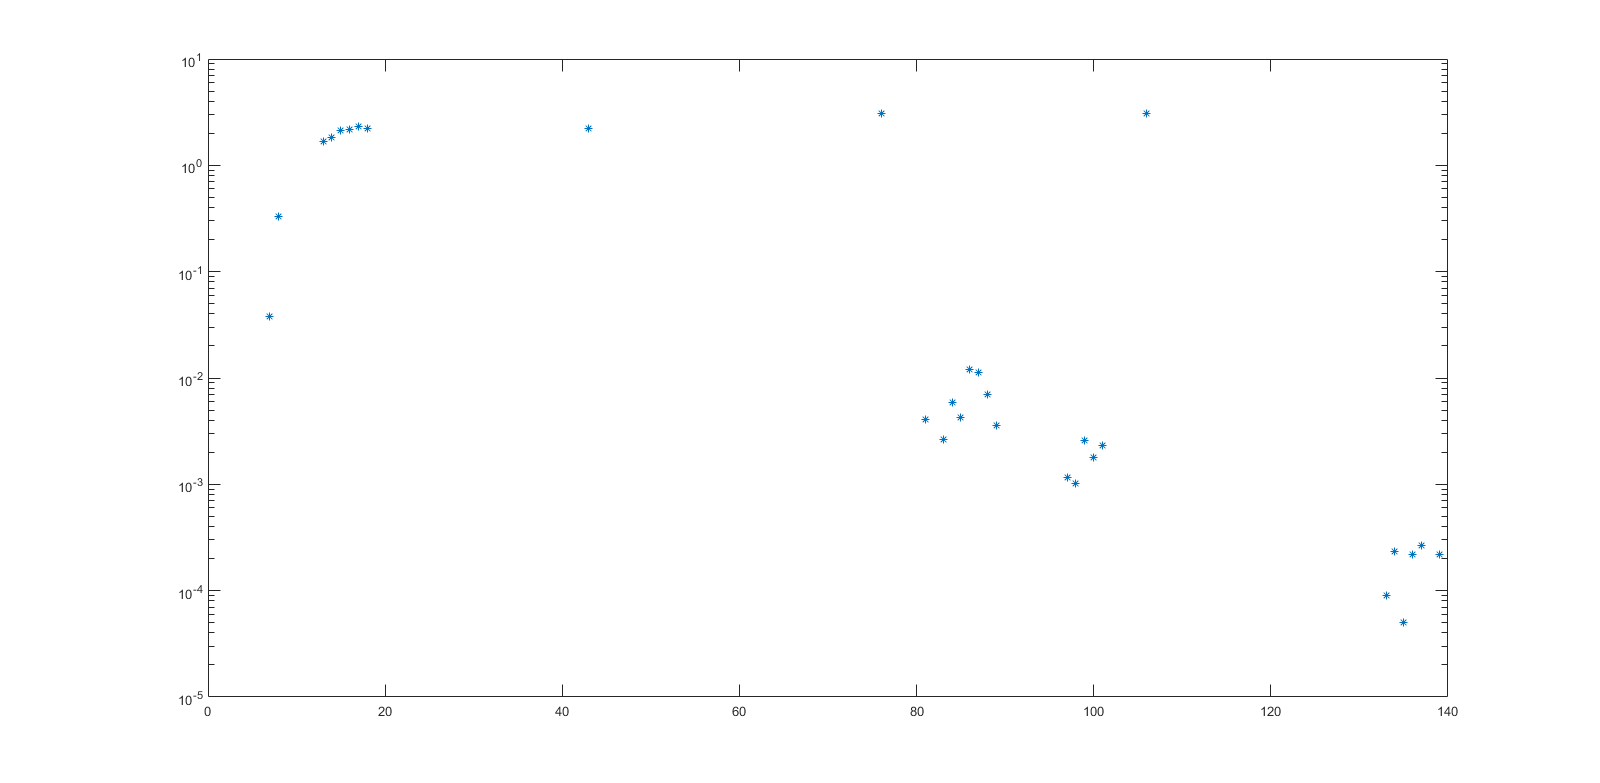
\includegraphics[width=0.5\textwidth]{Tekeningen/arnoldi_2_eig_150it}\label{arnoldi_2_150_it}}
\end{figure}

\begin{figure}[H]
  \centering
  \subfloat[arnoldi 3, 150 iteraties]{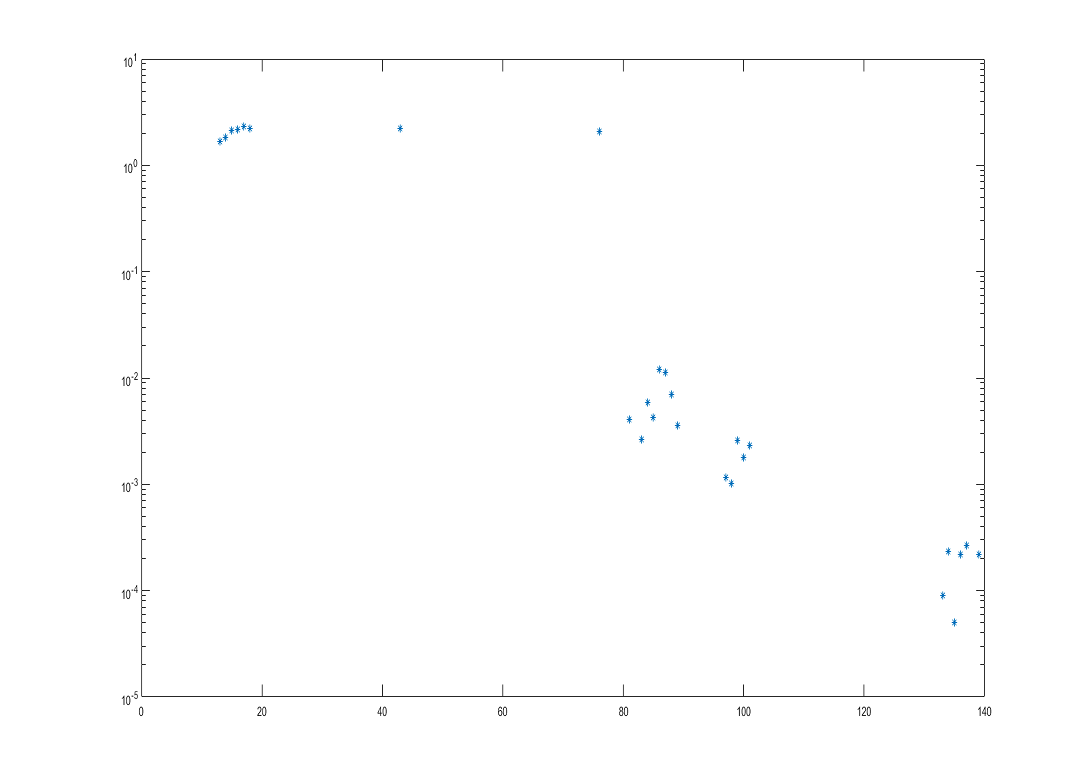
\includegraphics[width=0.5\textwidth]{Tekeningen/arnoldi_3_eig_150it}\label{arnoldi_3_150_it}}
  \hfill
  \subfloat[arnoldi 4, 150 iteraties]{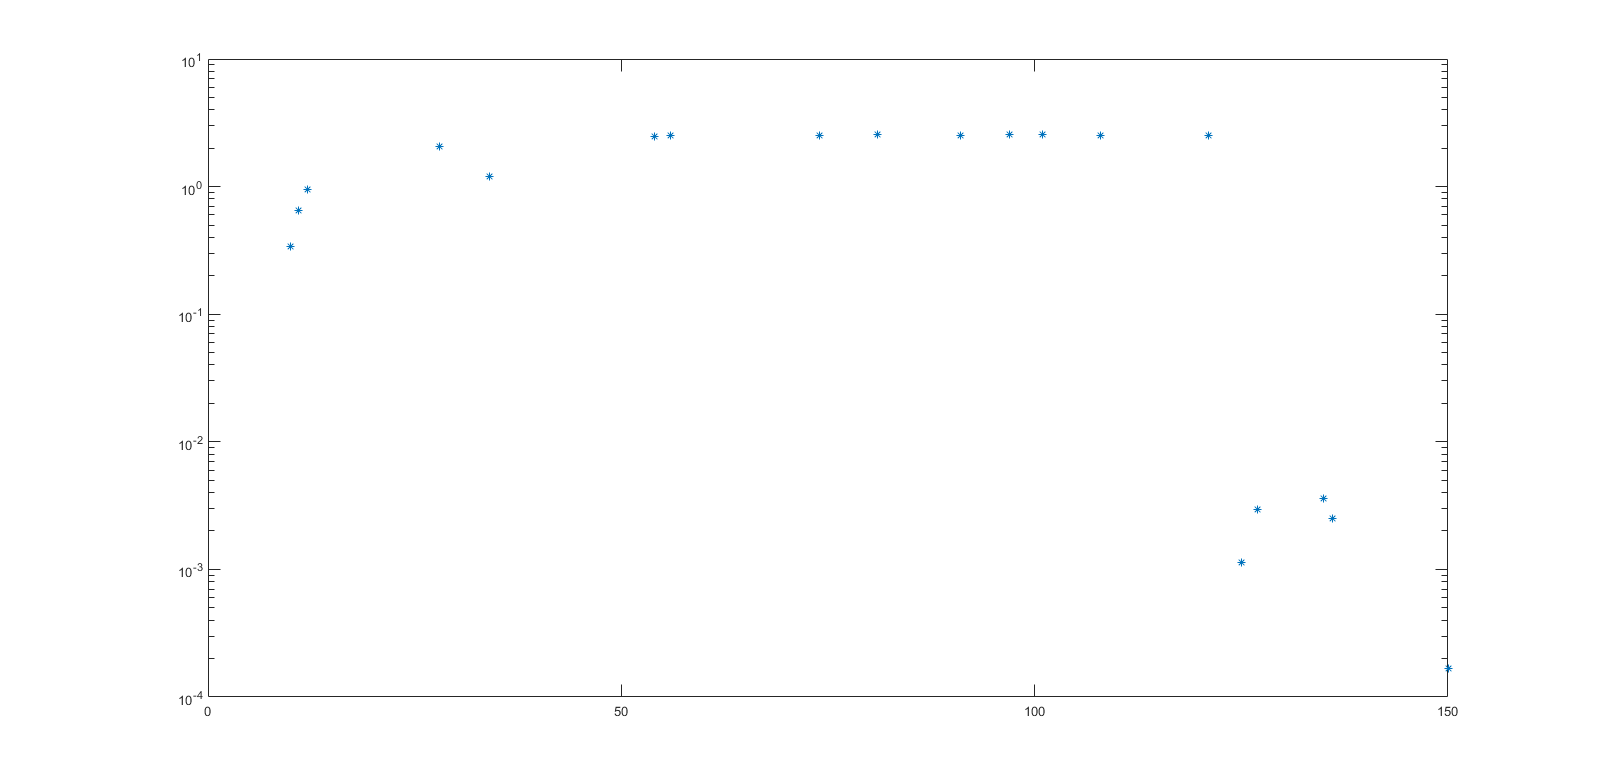
\includegraphics[width=0.5\textwidth]{Tekeningen/arnoldi_4_eig_150i}\label{arnoldi_4_150_it}}
\end{figure}